\documentclass{article}
\usepackage{a4wide}
\usepackage[margin=0.8in]{geometry}
\usepackage{graphicx}
\graphicspath{ {./} }

\begin{document}

\begin{titlepage}
\centering
\vspace*{6cm}
{\huge\bfseries BACnet Blocklists\par}

\vspace{3cm}

{\Large Introduction to Internet and Security}\\
\vspace{0.1cm}
{\Large FS 2021}\\
\vspace{0.1cm}
{\Large Universität Basel}

\vspace{1cm}

{\large Gruppe 12: Jannick Heisch, Paul Tr\"oger}

\vspace{1cm}

{\large 18.07.2021}

\end{titlepage}


\section{Introduction}
As an alternative to the normal centraliced internet secure scuttlebutt and BACnet implements similar features and tries to improve them. 
One such function that we have chosen as the subject of our project is blocklists.
We have looked at BACnet and realized that a content filter would be a useful function.
Blocking can have many reasons, for example harassment and inappropriate content.
We looked at what different ways of filtering content would be useful. 
Especially with regard to the structure of secure shuttlebutt.

\section{Background}
First we looked at what was already implemented in BACnet and how we could achive our goal with it.
Secure scuttlebutt events save the author of each message by saving their public key.
This identification of messages 
What can we filter?
We realized that the blocklist should be saved in a format that is easy to read and write to.
After looking into some options we decided on JSON because it is easy to use in python 
and because we used it before.

\section{Implementation}
Our finished module is meant to be used as a library.
Besides the code, two file types belong to it.
A blocklist used to save words and authors that should be blocked and
blocksettings which are used to change how things should be blocked.
The functions in our module can be used to edit and save blocklists and blocksettings.
As well as filter events, feeds and content.
It is also possible to share and import blocklists with the help of our module. 

\subsection{Documentation}
We decided early that a good documentation would be needed for our project.
Since it is build as a module that can be added to other projects, ease of use is very important.
Each function is commented in the code with the use of python comments. 

\subsection{Sharing Blocklists}
Blocklists can be shared with others. 
We provide functions to import and export these lists.

\subsection{Share Blocking}
With our module, it is not only possible to block words and authors from being displayed alone, but also to decide what should be shared with others.
A filter function can be called before a feed is shared. The functions goes through the feed and changes it if block words are found.
This can be toggled in the blocksettings.
It is also possible to share but not to see content with block words.

\subsection{Blocksettings}
With the blocksettings file you can change how content should be flitered and if it should be shared.
A user decides whether messages with a block word should be displayed but the word censored or whether the whole message should be removed.




\section{Result}

\subsection{Blocklist sharing}
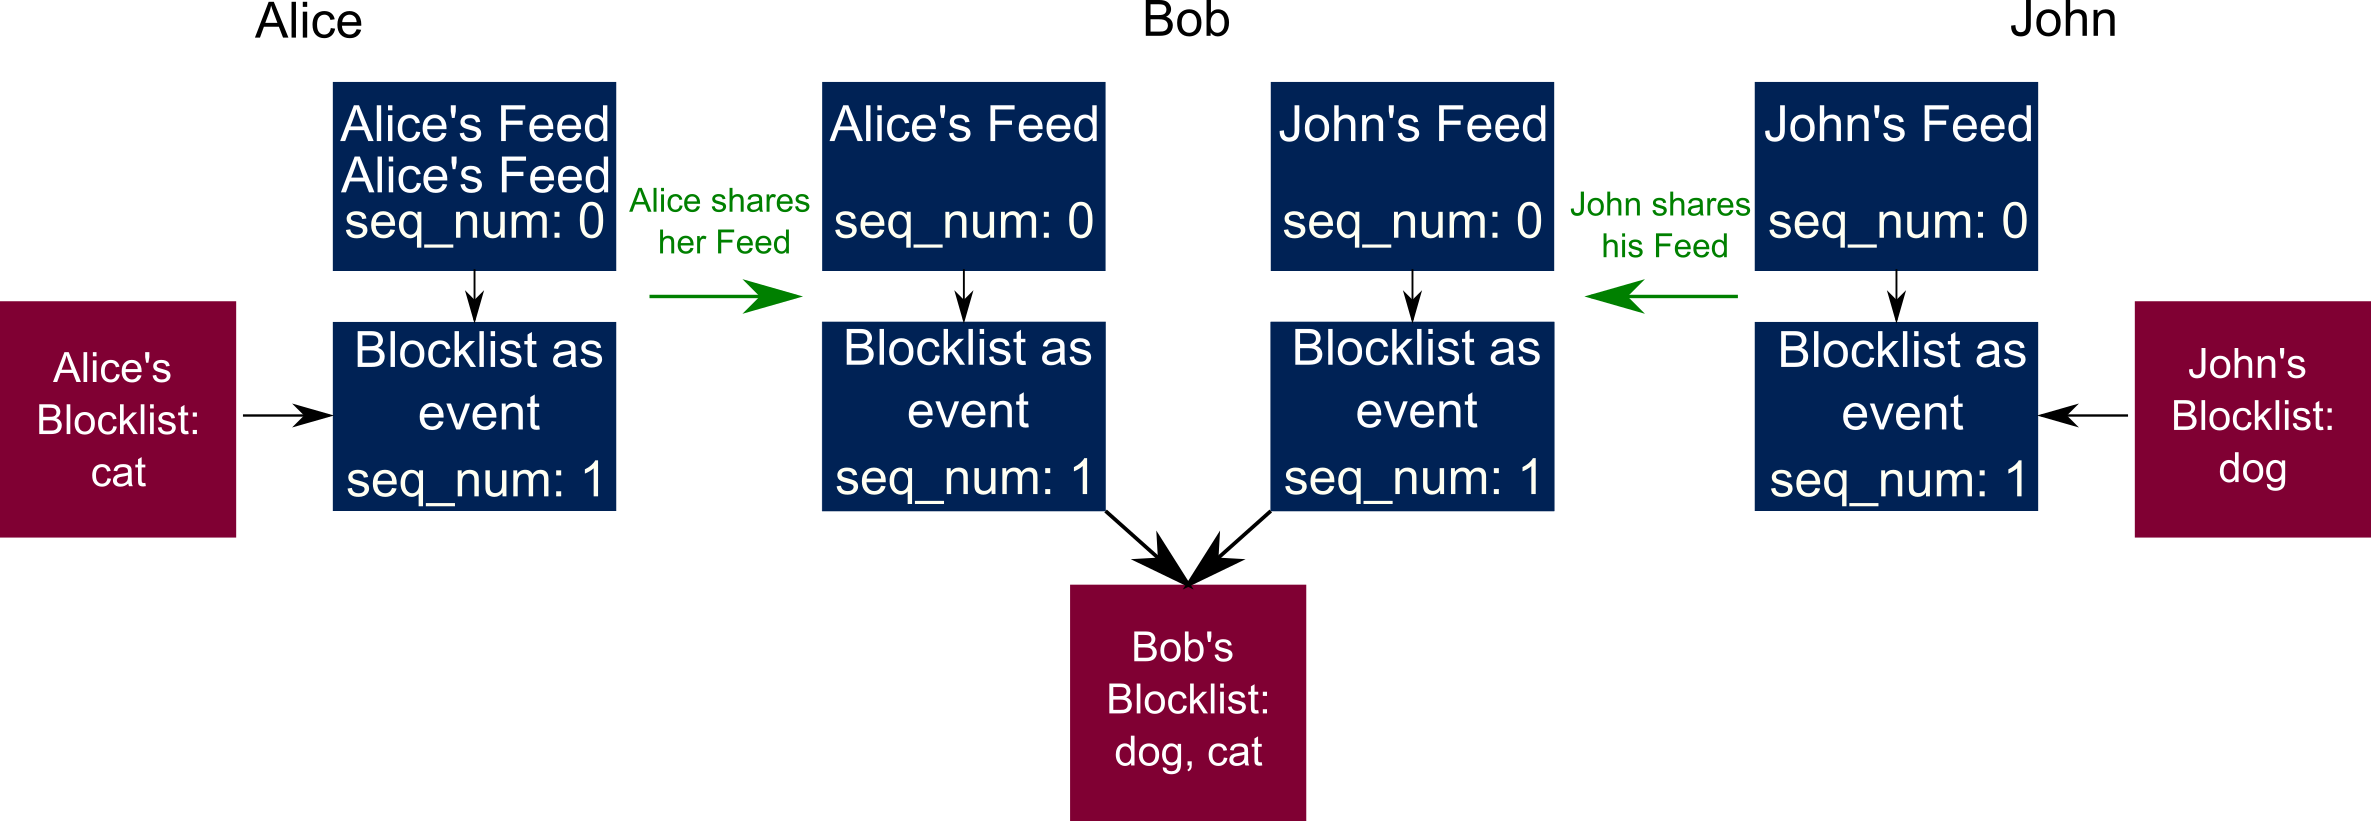
\includegraphics[width=\textwidth]{graph2}
This example shows how Blocklists can be shared over the secure scuttlebutt protocol.
The initial situation is that Bob does not yet have a block list. Alice and John, however, have two distinct ones.
Both Alice and John write their Blocklists into their feed.
After sharing them with Bob, he merges both Lists to use as his own.


\subsection{Suggested Blocking}
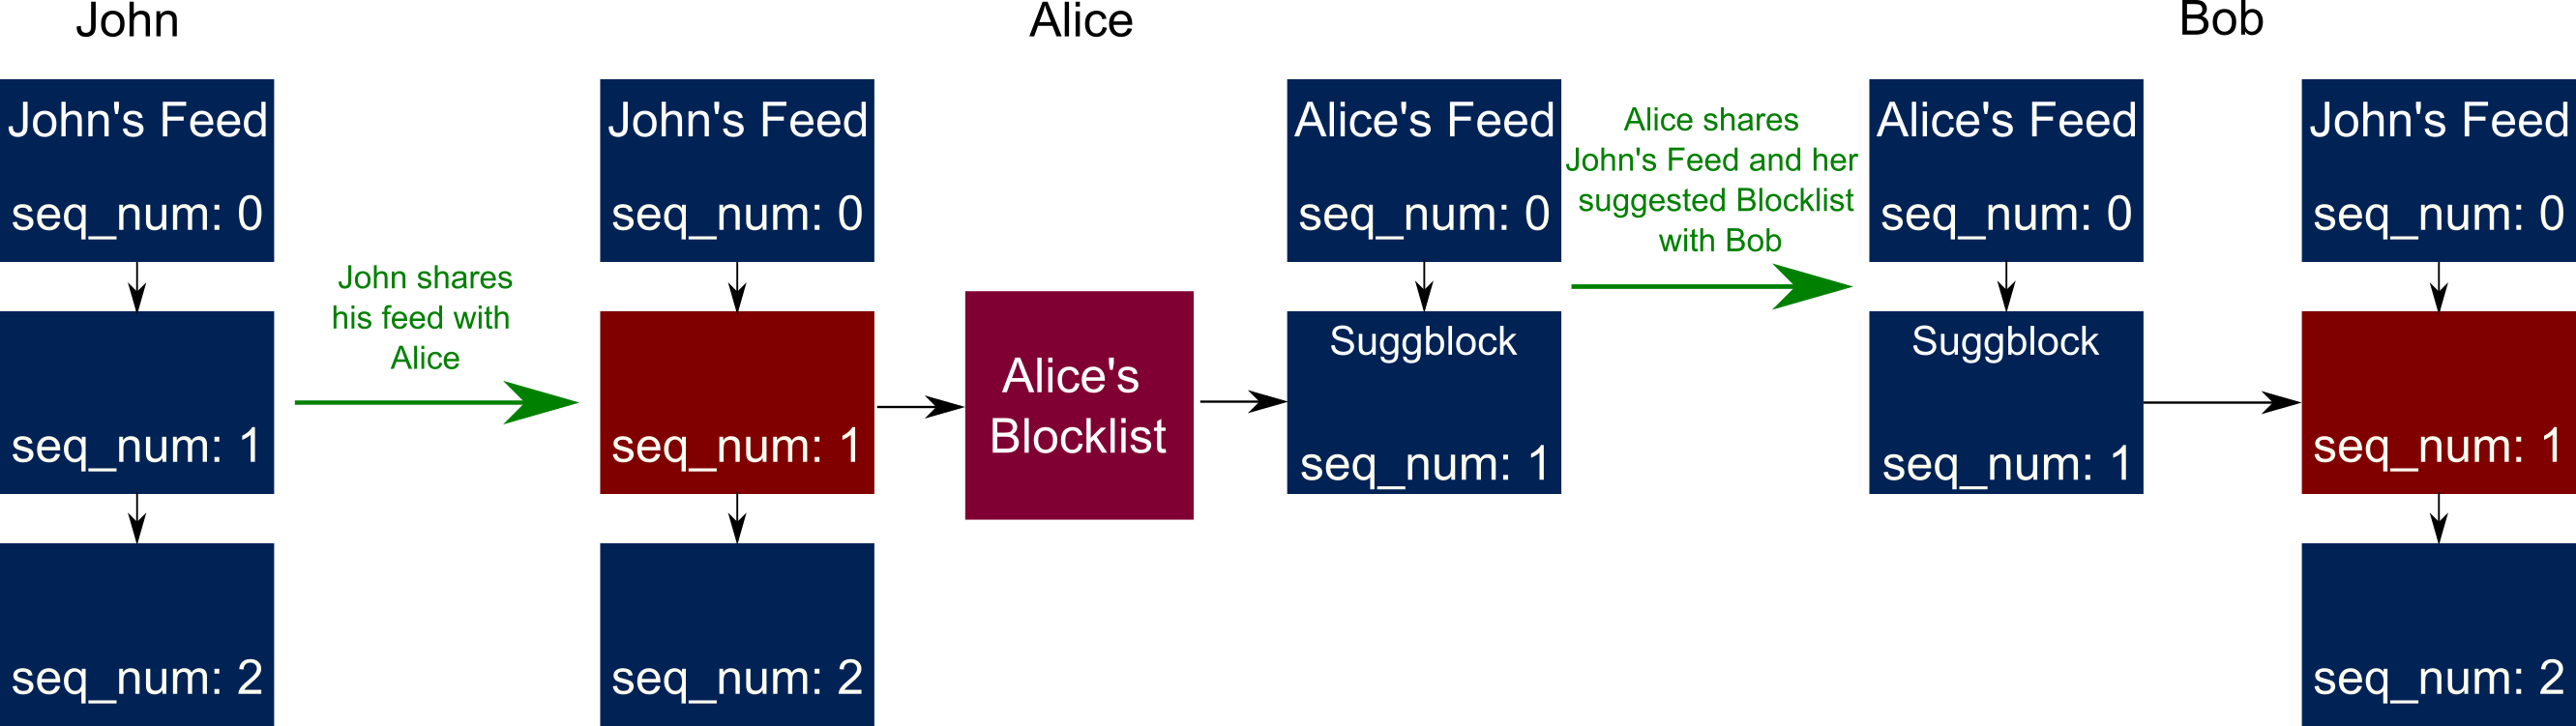
\includegraphics[width=\textwidth]{graph1}
Here you can see how someone can block entries from sharing them.
John sends his feed to Alice. Alice uses her own blocklist to determine that entry 1 should be blocked.
She writes a suggblock event into her own feed. Bob receives both Alice's and John's feed. 
With both he can use Alice's suggestion to block event 1 from John's feed.
Note that Bob does not need his own blocklist for this.






\section{Conclsion}
We hope our project can be used in future additions to BACnet to easily implement blocklists.
Like most projects, we had several versions until we got to our final code.
One of the biggest changes was to add a second file besides our block file to save all settings.


\section{Appendix}
\subsection{Used libraries}
\begin{itemize}
  \item JSON
\end{itemize}

\end{document}